%%%%%%%%%%%%%%%%%%%%%%%%%%%%%%%%%%%%%%%%%%%%%%%%%%%%%%%%%%%%%%%%%%%%%%%%%%%%%%%%
% Introduction
%%%%%%%%%%%%%%%%%%%%%%%%%%%%%%%%%%%%%%%%%%%%%%%%%%%%%%%%%%%%%%%%%%%%%%%%%%%%%%%%
\subsection{Introduction}
\label{fpga:introduction}
In the two decades since \glspl{FPGA} were introduced, they have radically
changed the way digital logic is designed and deployed \cite{Hauck:2007}. As
their capacity has grown and their architectures have incorporated specialized
features such as multipliers and distributed memories, \glspl{FPGA} have
increasingly found use as powerful parallel processing engines
\cite{Berkeley:2010}.

\glspl{FPGA} are revolutionary devices that offer a compromise between the
flexibility and ease of microprocessor-based software designs; and the
performance and efficiency of \gls{ASIC}-based hardware design. Unlike an
\gls{ASIC}, computations are programmed into the \gls{FPGA} device, instead of
being permanently constructed during the manufacturing process. This means that
an \gls{FPGA} device can be programmed and reprogrammed many times, allowing for
a significant level of flexibility whilst enabling a much faster and efficient
implementation than a software equivalent.

These benefits, however, do not come without a cost. Designing an
\gls{FPGA}-based system is a more complicated process than the development of a
software process. In order to effectively utilise hardware resources, the
designer of an \gls{FPGA}-based system must consider the hardware resources that
are provided by the \gls{FPGA} device, and must remain flexible during the
design process so as to utilise as many of the hardware resources that are
available whilst ensuring that the highest level of performance is obtained.
These considerations are seldom necessary in a pure-software approach, as tools
such as compilers and assemblers abstract the hardware implementation details
away from the developers in order to provide cross-system and, often,
cross-architecture compatibility.

Compared to an \gls{ASIC} design, which may take many months or years to design
and have a multimillion-dollar price tag, an \gls{FPGA} design might only take
days to create and cost tens to hundreds of dollars \cite{Hauck:2007}.

\begin{figure}
    \centering
    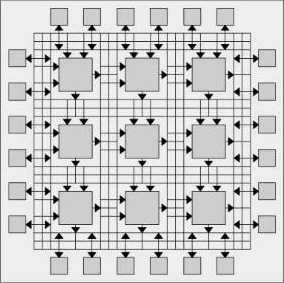
\includegraphics[width=0.5\textwidth]{fpga/abstract-view}
    \caption[An abstract view of an \gls{FPGA}]{An abstract view of an
        \gls{FPGA} \cite{Hauck:2007}}
    \label{fig:fpga:abstract}
\end{figure}

\autoref{fig:fpga:abstract} shows an abstract view of an \gls{FPGA}, which
consists of an \emph{array} of logic blocks (\emph{gates}) connected in a
general routing structure. The logic blocks contains processing elements for
implementing combinatorial logic, as well as flip-flops for implementing
sequential logic. The logic and routing elements of an \gls{FPGA} are controlled
by programming points, which may be based on Antifuse, Flash or \gls{SRAM}
technology. With the corresponding memory bits programmed, by way of a
configuration file or a bitstream, an \gls{FPGA} can be made to implement the
user's desired function. For this reason, \glspl{FPGA} are referred to as
\emph{field programmable} devices, as opposed to \emph{mask programmable}
devices, which have their  functionality fixed by masks during fabrication.

The design of an \gls{FPGA} program typically begins with an algorithm expressed
in a \gls{HDL} such as Verilog or \gls{VHDL}. An \gls{FPGA} design goes through
several development phases \cite{Hauck:2007}:
\begin{description}
    \item[Logic synthesis] Converts high level logic constructs and behavioural
        code into gates.
    \item[Technology mapping] Separate the gates into groupings that best match
        the \gls{FPGA}'s logic resources.
    \item[Placement] Assigns the logic groupings to specific logic blocks.
    \item[Routing] Determines the interconnect resources that will carry the
        user's signals.
    \item[Bitstream generation] Creates a binary file that sets all of the
        \gls{FPGA}'s programming points to configure the logic blocks and
        routing resources appropriately.
\end{description}

%%%%%%%%%%%%%%%%%%%%%%%%%%%%%%%%%%%%%%%%%%%%%%%%%%%%%%%%%%%%%%%%%%%%%%%%%%%%%%%%
% Device Architecture
%%%%%%%%%%%%%%%%%%%%%%%%%%%%%%%%%%%%%%%%%%%%%%%%%%%%%%%%%%%%%%%%%%%%%%%%%%%%%%%%
\subsection{Device Architecture}
\label{fpga:architecture}
Fundamentally, an \gls{FPGA} device consists of a large array of logic elements
(logic blocks) together with an interconnection network to pass data between
different logic blocks. A simplified representation illustrating the placement
of logic blocks and interconnections is shown in
\autoref{fig:fpga:architecture}.

\begin{figure}
    \centering
    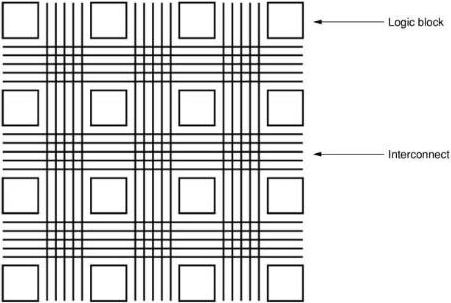
\includegraphics[width=0.5\textwidth]{fpga/architecture}
    \caption[A simplified representation of an \gls{FPGA} architecture]{A
        simplified representation of an \gls{FPGA} architecture
        \cite{Hauck:2007}}
    \label{fig:fpga:architecture}
\end{figure}

% Logic Elements
\subsubsection{Logic Blocks}
\label{fpga:architecture:logicBlocks}
Logic blocks are the fundamental component of any \gls{FPGA} architecture and
are made to realize a single logic function using a \gls{LUT} and a flip-flop.
The \glspl{LUT} provide the functional mapping between the logic block's input
and output bits. The flip-flop is a necessary sequential logic device for the
logic block to maintain a state. Almost all commercial \glspl{FPGA} have settled
on a \gls{LUT} as their basic building block \cite{Hauck:2007}.

From a circuit implementation perspective, a \gls{LUT} can be formed using a
$N:1$ multiplexer and an $N$-bit memory. In this implementation, the multiplier
simply maps some input combination of bits to some output combination of bits.
An important design consideration for an \gls{FPGA} is both the size of each
\gls{LUT} as well as the number of \glspl{LUT} that comprise a logic block.
These design considerations form the \emph{computational granularity} of the
\gls{FPGA}. Smaller (\emph{fine-grained}) \glspl{LUT} can effectively be used to
compute arithmetic and bit-level functions, but must be combined together in
order to realize more complicated functions. Larger (\emph{coarse-grained})
\glspl{LUT}, on the other hand, are capable of handling complicated logic
functions, at the cost of wasting logic resources when used to implement simple
logic functions.

\begin{figure}
    \centering
    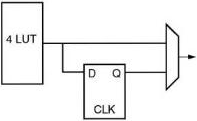
\includegraphics[width=0.5\textwidth]{fpga/logic-block}
    \caption[A simple \gls{LUT}-based logic block]{A simple \gls{LUT}-based
        logic block \cite{Hauck:2007}}
    \label{fig:fpga:logicBlock}
\end{figure}

% The Array and Interconnect
\subsubsection{The Array and Interconnect}
\label{fpga:architecture:arrayAndInterconnect}
Whilst the logic block is the fundamental component of an \gls{FPGA}, there is a
requirement for an interconnection network to allow data to flow between
adjacent (and possibly non-adjacent) logic blocks. This interconnection network
is known as the interconnect, and is a routing network that is configured to
route signals between logic blocks appropriately. Using this general design,
with enough logic blocks it is possible to perform any desired computation
\cite{Hauck:2007}.

Note that the interconnect structure shown in \autoref{fig:fpga:architecture} is
not representative of any actual interconnect structure that is currently in
use, but rather acts as a place holder for visual demonstration. In reality,
there are a wide range of methodologies relating to \gls{FPGA} interconnect
structure. Some of the more common configurations are described below.
\begin{description}
    \item[Nearest neighbour] Arguably the simplest interconnect structure, in
        which a logic block can communicate only with its immediate neighbours.
    \item[Segmented] A more generic and mesh-like interconnect structure. A
        logic block accesses nearby communication resources through a connection
        block, which itself allows logic block inputs and outputs to be assigned
        to arbitrary horizontal and vertical tracks. In addition, switch blocks
        connect converging routing tracks, allowing a signal on one track to
        communicate with a signal on another track.
    \item[Hierarchical] At the lowest level of the hierarchy, $2 \times 2$
        arrays of logic blocks are grouped together to form a single cluster.
        Within each cluster, only nearest-neighbour routing available. At each
        increasing level of the hierarchical interconnect structure, larger
        logic block clusters are formed. This interconnect structure exploits
        the property that a well-designed and well-placed circuit has mostly
        local connections and only a limited number of connections that need to
        travel long distances \cite{Hauck:2007}.
\end{description}

\begin{figure}
    \caption{\gls{FPGA} interconnect structures}
    \label{fig:fpga:interconnect}

    \centering
    \begin{subfigure}[b]{0.3\textwidth}
        \centering
        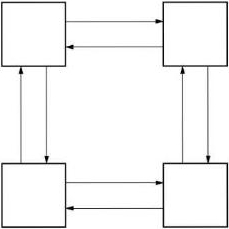
\includegraphics[width=\textwidth]{fpga/nearest-neighbour}
        \caption[Nearest neighbour interconnect structure]{Nearest neighbour
            interconnect structure \cite{Hauck:2007}}
        \label{fig:fpga:interconnect:nearestNeighbour}
    \end{subfigure}
    \quad
    \begin{subfigure}[b]{0.3\textwidth}
        \centering
        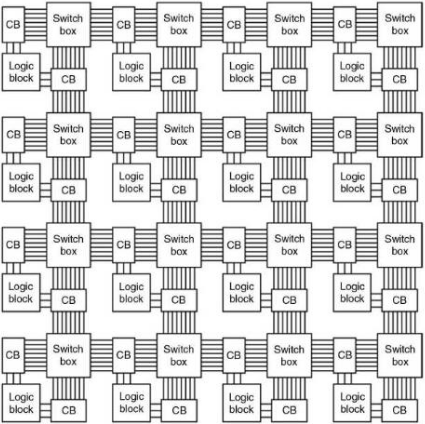
\includegraphics[width=\textwidth]{fpga/segmented}
        \caption[Segmented interconnect structure]{Segmented interconnect
            structure \cite{Hauck:2007}}
        \label{fig:fpga:interconnect:segmented}
    \end{subfigure}
    \quad
    \begin{subfigure}[b]{0.3\textwidth}
        \centering
        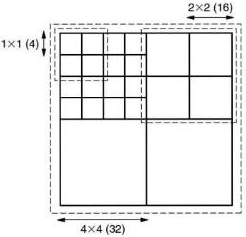
\includegraphics[width=\textwidth]{fpga/hierarchical}
        \caption[Hierarchical neighbour interconnect structure]{Hierarchical
            neighbour interconnect structure \cite{Hauck:2007}}
        \label{fig:fpga:interconnect:hierarchical}
    \end{subfigure}
\end{figure}

% Extended Logic Elements
\subsubsection{Extended Logic Elements}
\label{fpga:architecture:extendedLogic}
The aforementioned logic blocks of an \gls{FPGA} provide a useful foundation for
larger, more complicated, computational units including full adders and
multipliers. This augmentation is a methodology employed by \gls{FPGA}
architects, driven by application demands, to increase the versatility and
performance of \gls{FPGA} devices.

\paragraph{Adders}
\label{fpga:architecture:adders}
One fundamental operation that an \gls{FPGA} can be expected to perform is
addition. The simplest approach to implement a full-adder structure involves a
single logic block configured to compute the sum, together with a logic block
configured to compute the carry signal. Through this method, the cascading of
$N$ logic blocks can be used to implement an $N$-bit full adder
\cite{Hauck:2007}. The critical path of this design comes from the rippling
of the carry signal from lower-order bits to higher-order bits. This limitation
can be alleviated through placement considerations of the logic blocks, in such
a way as to minimise signal delay through the carry chain.

\paragraph{Multipliers}
\label{fpga:architecture:multipliers}
Another important operation that an \gls{FPGA} is expected to be able to compute
is that of multiplication. There are various implementations of a multiplier
that can be adopted, however in doing so the designer much choose between
lesser signal propagation delay and lesser logic block resources. For this
reason, it is not uncommon for \gls{FPGA} devices to provide dedicated
multiplier units implemented in silicon. In many cases, the performance and
power improvements offered by a dedicated multiplier warrant the silicon area
that would be required for such units.

\paragraph{Random Access Memory}
\label{fpga:architecture:ram}
Whilst it is possible to implement programmable memory using logic blocks,
it is a far more efficient use of \gls{FPGA} resources to provide dedicated
on-chip \gls{RAM} for this purpose. The grouping of banks of memory cells allows
for extremely fast lookup table operations, as well as providing memory
resources for queueing, buffering and general usage.

\paragraph{Processing Blocks}
\label{fpga:architecture:processor}
As the market for \gls{FPGA} devices extends to a wider range of applications,
it has become common for these devices to include general purpose processing
blocks embedded in their architecture. Whilst the parallel utilisation of
hardware resources provides performance improvements for pipelined and
vector-based operations, algorithms flows which are procedural and exhibit a
large amount of branching do not lend themselves readily to acceleration using
\glspl{FPGA}, and as such are much better performed on dedicated \glspl{CPU}
\cite{Hauck:2007}. The inclusion of processing blocks into \gls{FPGA} device
represents a significant movement supporting the use of \glspl{FPGA} as general
purpose, platform-orientated devices.

%%%%%%%%%%%%%%%%%%%%%%%%%%%%%%%%%%%%%%%%%%%%%%%%%%%%%%%%%%%%%%%%%%%%%%%%%%%%%%%%
% Configuration
%%%%%%%%%%%%%%%%%%%%%%%%%%%%%%%%%%%%%%%%%%%%%%%%%%%%%%%%%%%%%%%%%%%%%%%%%%%%%%%%
\subsection{Device Configuration}
\label{fpga:configuration}
In order to be configurable, and consequently reconfigurable, \glspl{FPGA} must
be programmed from some initial (blank) configuration to the final design
configuration for the project. The configuration process can essentially be
thought of as the construction of a flat binary file (known as a
\emph{bitstream}) which maps, bit-for-bit, to the programmable bits of the
\gls{FPGA} device. The configurable elements of an \gls{FPGA}, which are
configured through the bitstream, include the contents of a logic block (such as
the values resulting from a truth table), as well as the routing
interconnections.

There are various means by which an \gls{FPGA} can be configured, the most
common of which are outlined below.

% Static Random Access Memory
\subsubsection{Static Random Access Memory}
\label{fpga:configuration:sram}
\gls{SRAM} is volatile, static \gls{RAM} and is the most common method chosen
for device implementation, due to the potential it provides for fast and
infinite reconfiguration.

The main disadvantage of \gls{SRAM} is the power consumption necessary for such
hardware elements. This follows on from the volatile characteristic of the
memory, such that in the absence of a power source, the data on the storage
medium is not persistent.

% Flash Memory
\subsubsection{Flash Memory}
\label{fpga:configuration:flash}
Flash memory holds some improvements over \gls{SRAM} for the configuration of
\glspl{FPGA}, namely that the memory is non-volatile. This simplifies the
boot-up process by removing the necessity to re-download the bitstream at power
on. Flash memory, however, has a limited write cycle lifetime and often has
slower write speeds than \gls{SRAM}.

% Antifuse
\subsubsection{Antifuse}
\label{fpga:configuration:antifuse}
Antifuse is a metal-based link that behaves the opposite of a fuse
\cite{Hauck:2007}. Antifuse is initially in a `normally open' state, but through
a high-current programming process these links can be melted to form a circuit
connection. The clear disadvantage of Antifuse is that it is non-reprogrammable.
It does, however, have some distinct benefits over \gls{SRAM} and Flash memory:
\begin{itemize}
    \item Antifuse links can be made very small compared to \gls{SRAM} cells.
    \item It does not require any transistors.
    \item Low propagation delay across links.
    \item Zero static power consumption.
\end{itemize}